\documentclass[../main.tex]{subfiles}
\graphicspath{{\subfix{../images/}}}
\begin{document}

%%%%%%%%%%%%%%%%%%%%%%%%%%%%%%%%%%%%%%%%%%%%%%%%%%%%%%%%%%%%%%%%%%%%%%%%%%%%%%%%
\section{Основы работы с мультиметром}
\index{Электроника!Мультиметр}

Мультиметр -- незаменимый прибор, с его помощью можно узнать сопротивление
резистора, измерить напряжение, произвести проверку на проводимость
(``прозвонка''), узнать цвет и полярность светодиода и многое другое.

На рис. \ref{fig:multimeter-example} показан один из вариантов мультиметра.

\begin{figure}[ht]
  \centering
  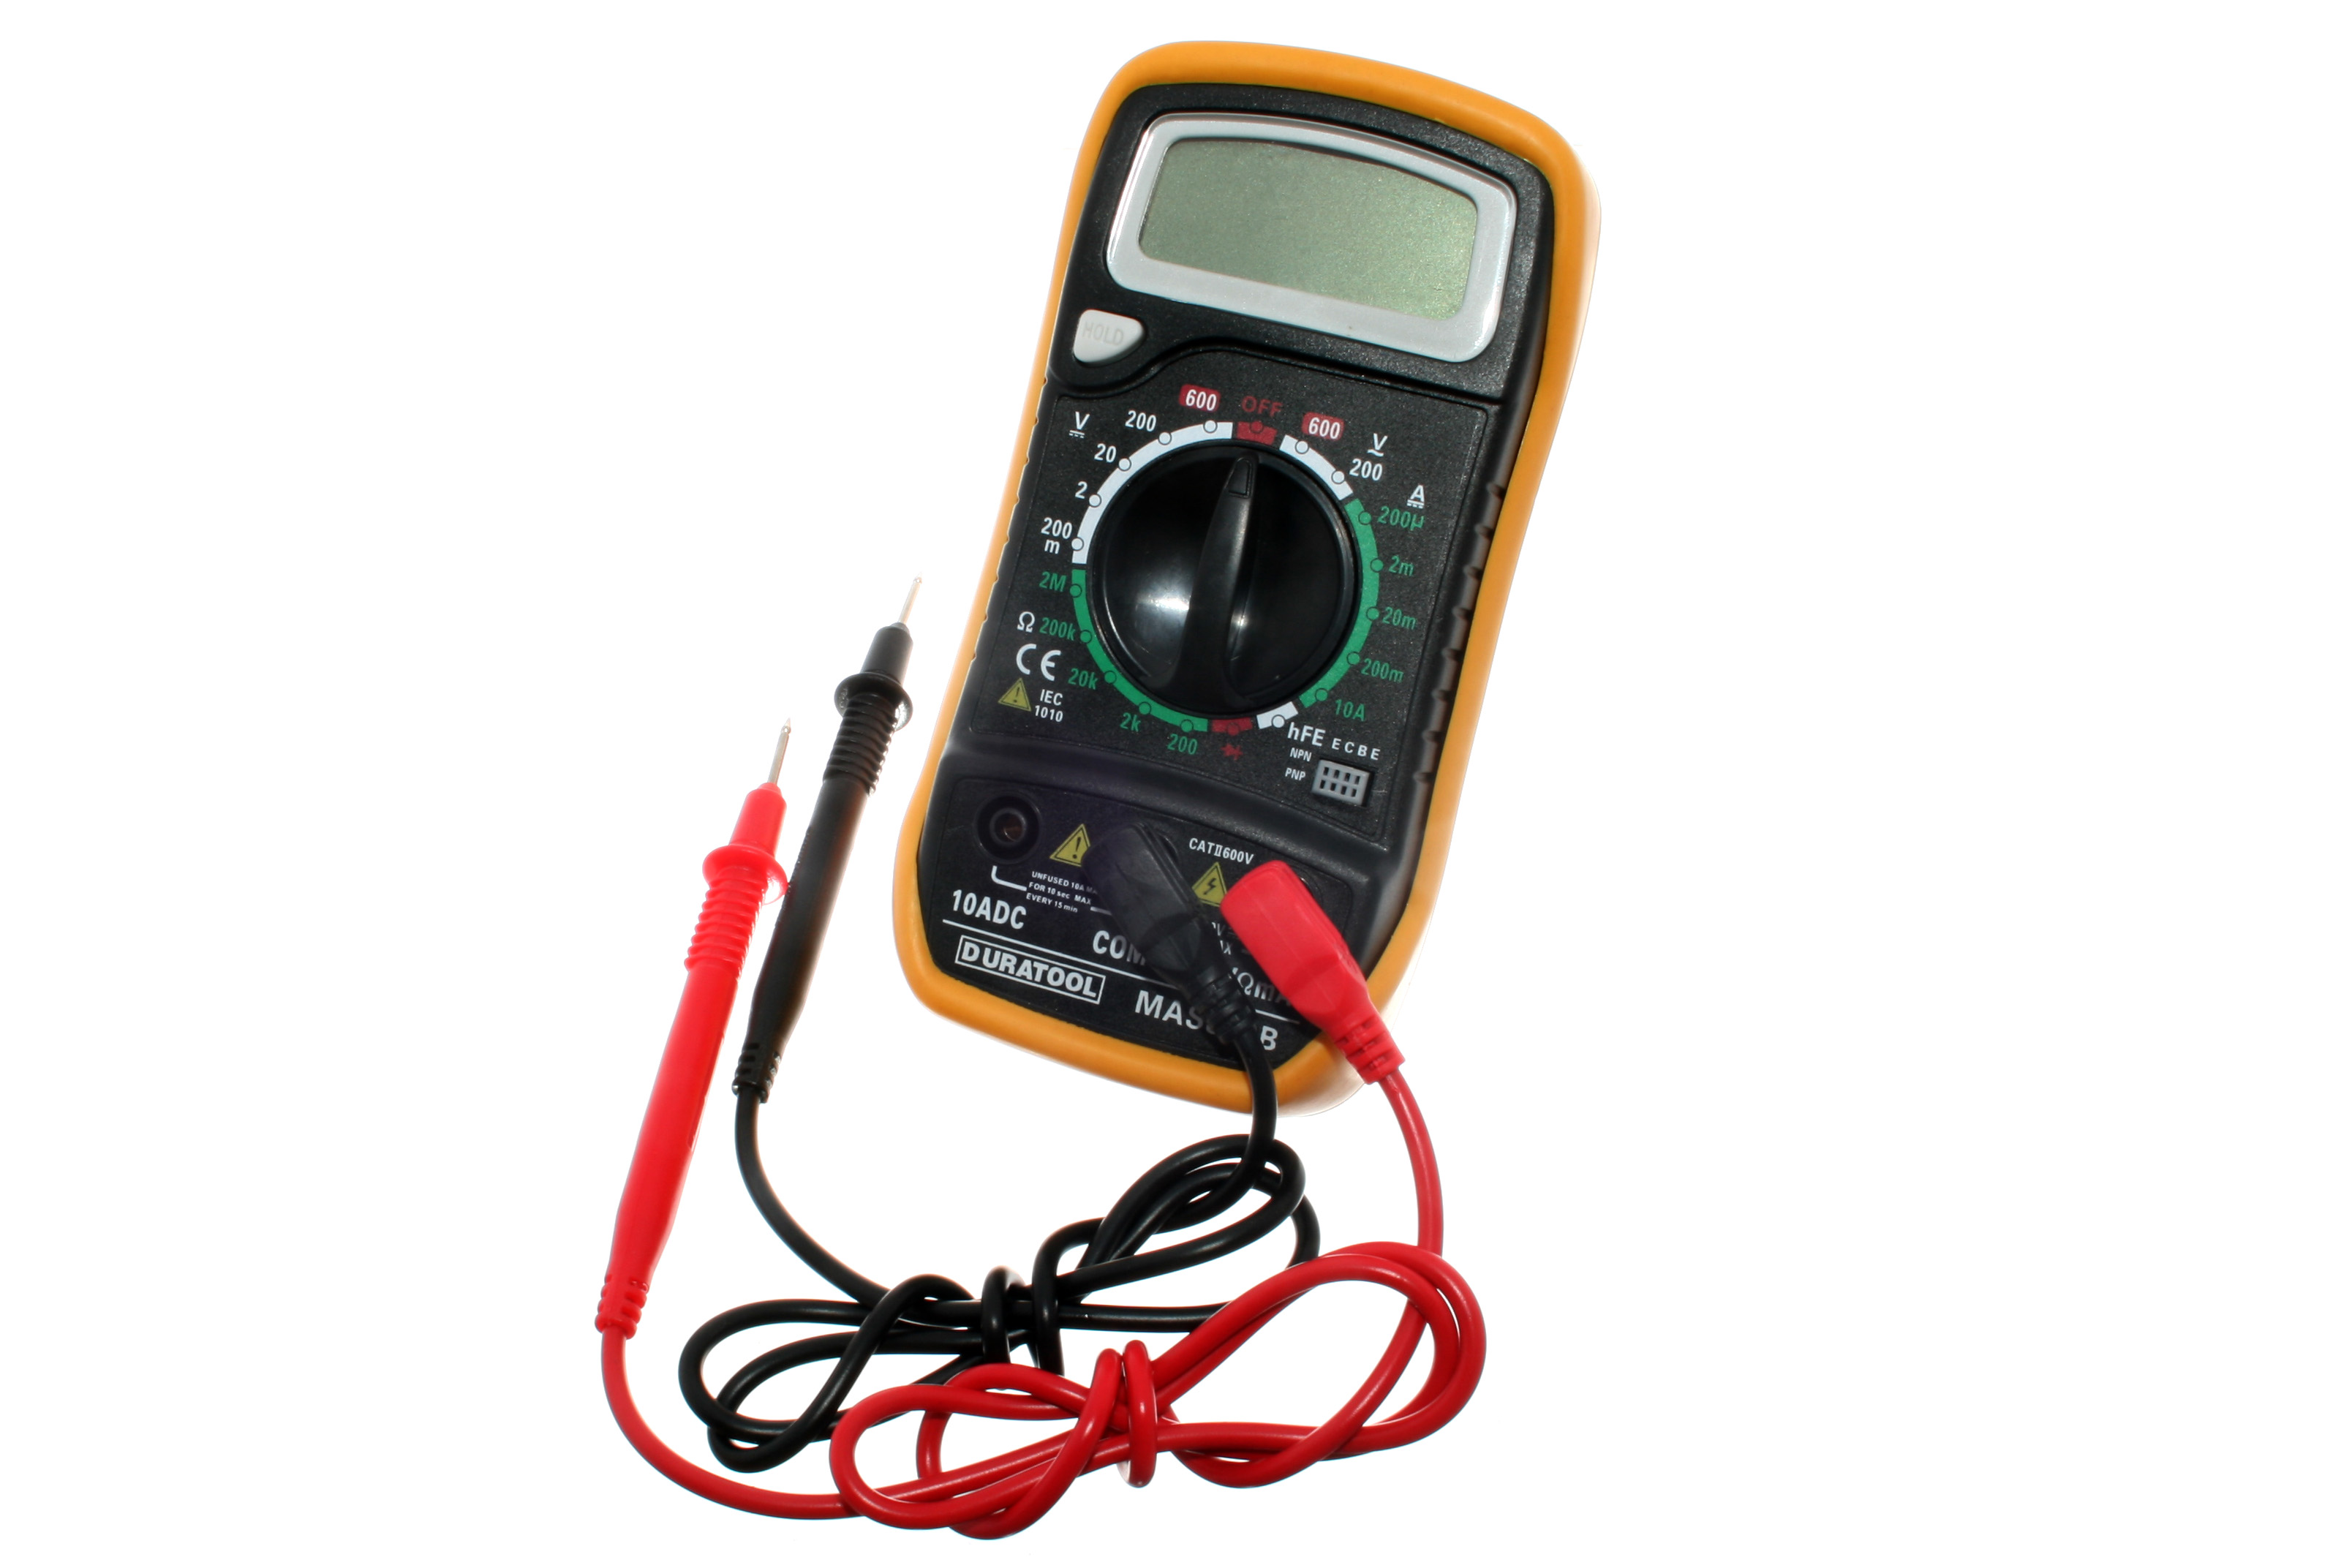
\includegraphics[width=14cm]{Digital_Multimeter}
  \caption{Пример мультиметра.}
  \label{fig:multimeter-example}
\end{figure}

\subsection{Основные параметры мультиметра}

Мультиметр измеряет текущее (мгновенное) значение параметров электронных
компонентов или же цепей.  В зависимости от модели, скорость ``реакции'' на
изменение параметров может отличаться, но как правило этот параметр не является
решающим.

Всего у мультиметров есть четыре\cite{fluke:multimeter} основных параметра:
\begin{itemize}
\item \textbf{Погрешность} (англ. \emph{accuracy}) определяет максимальную
  ошибку измерений.
\item \textbf{Прецезионность} (англ. \emph{precision}) позволяет достичь высокой
  повторяемости результатов замеров.
\item \textbf{Разрешение} (англ. \emph{resolution}) позволяет добиться большей
  точности измерений.
\item \textbf{Диапазон значений} (англ. \emph{range}) определяет, в каких
  диапазонах может быть измеряемый параметр.
\end{itemize}

Рассмотрим каждый из параметров подробнее.

Допустимая погрешность определяет наибольшую ошибку, которая может возникнуть в
специфических ситуациях использования устройства.  Этот параметр определятеся в
процентах и показывает, как близко полученное с помощью устройства значение к
фактическому (стандартному) значению измеряемого сигнала.  Данный параметр
задаётся в процентах, чем меньше значение -- тем лучше.

Показание прецезионности определяет способность мультиметра регулярно
воспроизводить близкие друг к другу показания.  При этом устройство с высокой
допустимой погрешностью будет давать показания, явно отличные от фактических
измеряемых значений, однако при хорошей прецензионности разброс показаний будет
минимальным.

Если устройство обладает низкой погрешностью и высокой прецезионностью, то тогда
показания будут близки к фактическим и при повторных замерах они будут близки
друг к другу.

Разрешение определяет наименьший шаг, с которым измерительный инструмент может
произвести замер.  Предположим, что мы измеряем напряжение на стандартной 1.5В
батарее.  Если цифровой мультиметр имеет разрешение 1мВ в диапазоне измерений
3В, то можно будет увидеть изменение напряжения на 1мВ при замерах.  Таким
образом, пользователь сможет увидеть изменение на одну тысячную вольта, или
0.001В в диапазоне 3В.

Диапазон значений часто связан с разрешением, и иногда указывается в
спецификации на устройство.  Большинство мультиметров имеют авто-определение
диапазона измерений, что позволяет им автоматически выбирать подходящий диапазон
для измеряемого значения.  Если диапазон значений меньше измеряемого значения,
то цифровые мультимеры как правило тем или иным способом уведомляют о
перегрузке.  Наиболее точные измерения выполняются на наименьшем диапазоне
значений, который позволяет измерять сигнал без ухода в перегрузку.

\subsection{Условные обозначения на мультиметре}

Далее приведена таблица на которой отражены основные символы, встречающиеся на
корпусе прибора, необходимые для работы с мультиметром:

\begin{tabular}{| m{8em} | m{22em} |}
  \hline
  \textbf{Обозначение} & \textbf{Описание} \\
  \hline
  V$\sim$ & Измерение напряжения переменного тока. \\
  \hline
  mV$\sim$ & Измерение напряжения переменного тока, милливольты (мВ.) \\
  \hline
  V\textdirectcurrent{} & Измерение напряжения постоянного тока. \\
  \hline
  mV & Измерение напряжения постоянного тока, милливольты (мВ.) \\
  \hline
  A\textdirectcurrent{} & Измерение постоянного тока. \\
  \hline
  A$\sim$ & Измерение переменного тока. \\
  \hline
  $\Omega$ & Измерение сопротивления. Как правило, доступны следующие диапазоны:
  ``2k'' (2000 Ом), ``20k'' (20000 Ом), ``200k'' (200000 Ом) и ``2M'' (два
  мегаома, или два миллиона Ом.)\\
  \hline
  HOLD & ``Заморозить'' текущее показание на дисплее. \\
  \hline
  \esymbol{diode} & Тестирование диодов. \\
  \hline
  Hz   & ``Hertz'', Герцы -- измерение частоты. \\
  \hline
  \esymbol{capacitor} & Измерение ёмкости. \\
  \hline
  \soundWaveIcon{} & Измерение целостности цепи (так называемая ``прозвонка''.) \\
  \hline
  hFE & ``\textbf{H}ybrid parameter \textbf{f}orward current gain, common
  \textbf{e}mitter'' -- режим тестирования транзисторов. \\
  \hline
\end{tabular}

%% TODO: Добавить описание функций мультиметра.

\experiment{0} { Попробуйте померять с помощью мультиметра сопротивление
  резисторов, соединяя их последовательно и параллельно через макетную плату.
  Как меняется сопротивление собранной цепи? }

\experiment{1} { Померяйте сопротивление других проводников -- например, проводов
  для макетной платы Arduino, металлических предметов. Какое у них
  сопротивление?}

\experiment{2} { Известно, что графит является проводником. Померяйте
  сопротивление графитового стержня в карандаше.  Также попробуйте на листе
  бумаги нарисовать жирную графитовую линию и померяйте её сопротивление.  Какое
  сопротивление вы видите? }

\end{document}
